\chapter{Western Contact and the Nineteenth Century}

\section{The problem}

Between 1839 and 1876 all three East Asian states were forced by Western gunboats (and,
in Korea's case, by Japanese ones) to accept \emph{treaties} on Western terms. The
question for this week: \emph{why did Japan respond by rapidly modernizing and becoming
an imperial power, while Qing China and Joseon Korea did not?} The professor warned us
against the old answer (``Japan was flexible, China and Korea were stuck in Confucian
tradition'') and asked us to look at structures, timing and contingency.

\section{China: the Opium Wars and the ``century of humiliation''}

\subsection{The Canton system}

From 1757 the Qing restricted Western trade to one port, Canton (Guangzhou), where
foreign merchants could deal only with licensed Chinese firms (the \emph{Cohong}). The
Macartney embassy (1793) asked for wider trade and diplomatic representation;
the Qianlong emperor replied that China possessed all things and had no need of British
manufactures. Western historians long quoted this as proof of Chinese arrogance; more
recent work shows the Qing were well informed and that the letter fitted tributary
conventions.

\subsection{Opium}

Britain bought large quantities of tea and paid in silver. To reverse the flow, the East
India Company grew opium in Bengal and sold it to private traders who smuggled it into
China. By the 1830s silver was flowing \emph{out} of China, and addiction was widespread.

\begin{center}
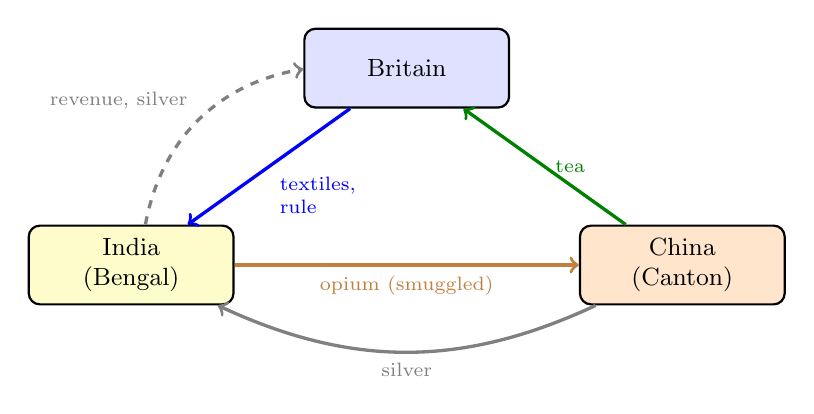
\begin{tikzpicture}[n/.style={draw, thick, rounded corners, minimum width=2.6cm, minimum height=1cm, align=center, font=\small}]
  \node[n, fill=blue!12] (br) at (0,2.5) {Britain};
  \node[n, fill=yellow!20] (in) at (-3.5,0) {India\\(Bengal)};
  \node[n, fill=orange!20] (cn) at (3.5,0) {China\\(Canton)};
  \draw[->, very thick, brown] (in) -- node[below, font=\scriptsize] {opium (smuggled)} (cn);
  \draw[->, very thick, gray] (cn) to[bend left=25] node[below, font=\scriptsize] {silver} (in);
  \draw[->, very thick, green!50!black] (cn) -- node[right, font=\scriptsize] {tea} (br);
  \draw[->, very thick, blue] (br) -- node[below right, font=\scriptsize, align=left] {textiles,\\rule} (in);
  \draw[->, very thick, gray, dashed] (in) to[bend left=35] node[above left, font=\scriptsize] {revenue, silver} (br);
\end{tikzpicture}
\end{center}

\subsection{First Opium War (1839--1842)}

The commissioner \textbf{Lin Zexu} confiscated and destroyed over 20\,000 chests of opium in
1839 and wrote to Queen Victoria asking how Britain would feel if foreigners sold poison
in England. Britain responded with a naval expedition. Steam gunboats like the
\emph{Nemesis} proved decisive.

\begin{important}[Treaty of Nanjing (1842) -- the first ``unequal treaty'']
\begin{itemize}
  \item Hong Kong island ceded to Britain.
  \item Five treaty ports opened (Canton, Amoy/Xiamen, Fuzhou, Ningbo, Shanghai).
  \item Indemnity of 21 million silver dollars; fixed low tariffs.
  \item Supplementary treaties: \textbf{extraterritoriality} (foreigners tried in their own
        consular courts) and the \textbf{most-favoured-nation} clause (any privilege given
        to one power goes to all).
\end{itemize}
\end{important}

\subsection{Mid-century crises}

\begin{itemize}
  \item \textbf{Second Opium (Arrow) War} (1856--1860): British and French troops took
        Beijing and burned the Summer Palace; opium legalized; more ports; missionaries
        allowed inland; Russia took the territory around Vladivostok.
  \item \textbf{Taiping Rebellion} (1850--1864): led by Hong Xiuquan, a failed examination
        candidate who believed he was the younger brother of Jesus. The Taiping
        ``Heavenly Kingdom'' ruled from Nanjing for over a decade; perhaps 20--30 million
        died, making it the deadliest civil war of the 19th century. It was suppressed by
        regional armies led by Confucian officials such as Zeng Guofan, not by the Manchu
        banners, a shift of power to the provinces.
\end{itemize}

\subsection{Self-Strengthening (1861--1895)}

Officials such as Zeng Guofan, Li Hongzhang and Prince Gong built arsenals, shipyards and a
foreign-language school under the slogan ``Chinese learning as the essence, Western
learning for practical use'' (\zht{中體西用}). The movement produced a modern navy, but it
was regionally fragmented, opposed at court, and starved of funds (the Empress Dowager
Cixi diverted naval money to rebuild the Summer Palace, a story that may be exaggerated).
Defeat by Japan in 1895 revealed its limits.

\section{Japan: from Perry to Meiji}

\subsection{The arrival of the ``black ships''}

In 1853 US Commodore \textbf{Matthew Perry} sailed into Edo Bay with steam warships and
demanded that Japan open its ports. He returned in 1854 and obtained the Treaty of
Kanagawa. The Harris Treaty (1858) and similar treaties with other powers gave
extraterritoriality and fixed tariffs, as in China.

\begin{aside}
Japanese officials had been reading Dutch reports about the Opium War. They knew what had
happened to China, which is one reason the bakufu chose to negotiate rather than fight.
Information mattered.
\end{aside}

\subsection{Collapse of the bakufu}

\begin{enumerate}
  \item Signing the treaties without imperial approval discredited the shogun.
  \item Activists rallied around the slogan ``Revere the emperor, expel the barbarians''
        (\ja{尊王攘夷}, sonnō jōi).
  \item Two powerful \emph{tozama} domains, \textbf{Satsuma} and \textbf{Chōshū}, tried to
        expel foreigners, were bombarded by Western ships (1863--64), and concluded that
        they must first modernize.
  \item Satsuma and Chōshū allied (1866), defeated bakufu forces, and in January 1868
        proclaimed the ``restoration'' of imperial rule. The Boshin War (1868--69) ended
        resistance.
\end{enumerate}

\subsection{The Meiji Restoration}

The teenage Emperor Mutsuhito took the reign name \emph{Meiji} (\ja{明治}, ``enlightened
rule''). Power actually lay with an oligarchy of young samurai from the victorious domains
(Ōkubo Toshimichi, Kido Takayoshi, Itō Hirobumi, Yamagata Aritomo).

\begin{center}
\begin{tabular}{lp{10.5cm}}
\toprule
Year & Reform \\
\midrule
1868 & Charter Oath: assemblies, abolish ``evil customs'', seek knowledge throughout the world \\
1871 & domains abolished, replaced by prefectures; Iwakura Mission to the US and Europe (1871--73) \\
1872 & universal primary education; first railway (Tokyo--Yokohama); solar calendar \\
1873 & conscription; land tax reform \\
1876 & samurai stipends ended; samurai forbidden to wear swords \\
1877 & Satsuma Rebellion of Saigō Takamori crushed by conscript army \\
1889 & Meiji Constitution (Prussian model): sovereign emperor, Diet with limited powers \\
1890 & Imperial Rescript on Education (loyalty, filial piety, service to the state) \\
1894--99 & unequal treaties revised (extraterritoriality ended) \\
\bottomrule
\end{tabular}
\end{center}

\begin{important}[Slogans of Meiji]
\begin{itemize}
  \item \ja{富国強兵} (fukoku kyōhei): ``rich country, strong army''.
  \item \ja{文明開化} (bunmei kaika): ``civilization and enlightenment'' (Western dress,
        beef eating, brick buildings in Ginza).
  \item \ja{和魂洋才} (wakon yōsai): ``Japanese spirit, Western technique'' -- compare
        China's \zht{中體西用}.
\end{itemize}
\end{important}

\section{Korea: the ``hermit kingdom'' opened}

\begin{itemize}
  \item The regent \textbf{Heungseon Daewongun} (ruled for his son King Gojong, 1864--1873)
        persecuted Catholics (1866) and repelled French (1866) and American (1871)
        expeditions, erecting stones that warned against peace with Western barbarians.
  \item \textbf{Treaty of Ganghwa} (1876): Japan, using Perry's methods, forced Korea to open
        ports and accept extraterritoriality. Japan declared Korea an ``independent state'',
        meaning independent of Chinese suzerainty.
  \item Korea became a contested arena: Qing China (Yuan Shikai as resident in Seoul),
        Japan and Russia competed for influence. Reformers like Kim Ok-gyun (Gapsin Coup,
        1884) looked to Meiji Japan as a model and failed.
  \item \textbf{Donghak Rebellion} (1894): a peasant uprising inspired by the syncretic
        ``Eastern Learning'' religion. Both China and Japan sent troops.
\end{itemize}

\section{The Sino-Japanese War (1894--95)}

Japan quickly defeated Qing armies in Korea and destroyed the Beiyang fleet. The
\textbf{Treaty of Shimonoseki} (1895):

\begin{itemize}
  \item China recognized Korean ``independence'' (ending the tributary relationship);
  \item ceded \textbf{Taiwan} and the Liaodong peninsula to Japan (Russia, France and
        Germany forced Japan to return Liaodong: the ``Triple Intervention'');
  \item paid a large indemnity, which funded Japanese industrialization.
\end{itemize}

\begin{remark}
1895 overturned the regional order of two thousand years: the former student had defeated
the teacher. Chinese students soon went to Tokyo in their thousands to learn how Japan had
done it.
\end{remark}

\section{Why did the outcomes differ?}

\begin{center}
\begin{tabular}{p{3.6cm}p{4.6cm}p{4.6cm}}
\toprule
Factor & Japan & China \\
\midrule
Size and unity & compact, ethnically homogeneous, easier to reform & vast; Manchu minority dynasty wary of Han Chinese power \\
Timing & opened 1854, after seeing China's defeat & first to be hit; reforms only after enormous internal rebellion \\
Elite & samurai (warriors, many impoverished) had little to lose & examination elite whose status rested on classical learning \\
Political structure & bakufu could be overthrown by domains in the emperor's name & dynasty's legitimacy tied to the Confucian order \\
Prior knowledge & Dutch learning; decentralised domains experimenting & strong but more insulated scholarly tradition \\
\bottomrule
\end{tabular}
\end{center}

\begin{important}[Exam essay tip]
The professor's preferred structure: (1) challenge the ``tradition vs.\ modernity''
framing; (2) compare at least three structural factors; (3) mention contingency (e.g.\ the
Taiping Rebellion, the death of key leaders); (4) note that Japan's ``success'' included
becoming an imperialist power, which is not simply a happy ending.
\end{important}

\section*{Summary}
\begin{itemize}
  \item Opium Wars (1839--42, 1856--60) and the unequal treaty system: treaty ports,
        extraterritoriality, tariffs, indemnities.
  \item Taiping Rebellion devastated China and shifted power to provinces;
        Self-Strengthening was partial.
  \item Perry (1853--54) led to the collapse of the bakufu and the Meiji Restoration (1868):
        centralization, conscription, education, constitution.
  \item Korea was opened by Japan in 1876 and became the object of rivalry.
  \item 1895 Treaty of Shimonoseki: Japan gains Taiwan and ends China's tributary claim to
        Korea.
\end{itemize}
